\subsection{Goals}
\label{subsec:exp:goals}
\noindent The main goal of conducted experimental evaluation was to verify the impact of \emph{given budget} and \emph{treshold} values on overall classification accuracy, measured for each processed chunk, with the aim to calibrate parameters in a way that (a) reduces usage of labels (b) without classification accuracy deterioration.

\subsection{Setup}
\label{subsec:exp:setup}

\subsubsection{Software environment}

\noindent Most of the research devoted to \emph{data streams} is currently conducted using the \textsc{moa} environment \cite{Bifet:2010}, implemented in the \emph{Java} programming language. It includes a collection of base classifiers, necessary experimental methods, measurement tools and, above all, data stream generators. Knowing a growing tendency to employ \emph{scikit-learn} library \cite{scikit-learn}, it was decided to use it in implementation of the method described in following paper. It is not widely used with data streams, however, the potentiality of such processing was confirmed by a short article with a \emph{proof-of-concept} available in the on-line \emph{scikit-learn} documentation\footnote{\url{http://scikit-learn.org/stable/modules/scaling_strategies.html}}. 

It was necessary to create a new experimental flow for processing streams, enhanced with a class used to control a learning process. Current state of \emph{scikit-learn} library allows to process data streams using classifiers having implemented the \emph{partial fit} method, nevertheless as we mentioned above, we would like to employ inbuilt forgetting mechanism used by neural networks, therefore we used the implementation of \emph{\textsc{mlp}} --- Multi-layer Perceptron classifier, optimizing the log-loss function using \textsc{lbfgs} (\emph{Limited memory Broyden–-Fletcher–-Goldfarb–-Shanno}) algorithm \cite{Mokhtari:2015}.

The implementation of the active approach described in this paper as well as the workflow of learning from data streams using the \emph{scikit-learn} library are part of the \emph{stream-learn} module being developed by our research team\footnote{\url{https://github.com/w4k2/stream-learn}}. Full code of experiments and presented examples, together with extended research results, can be found in the article repository\footnote{\url{https://github.com/w4k2/active_learning}}.

\subsection{Benchmark data streams}

\noindent The pool of analyzed data consist of \oldstylenums{12} streams:


\begin{itemize}
	\item Three real streams:
    \begin{itemize}
    \item \emph{covtypeNorm} dataset \cite{Frank:2010} includes the observations which may be used to classify the cover type of a forest on the basis of cartographic variables. It contains \oldstylenums{54} attributes and \oldstylenums{7} class labels. The appearance of the concept drift is a result of the changes in geographical condition.
\item \emph{clecNormNew} (electricity) dataset \cite{Harries:1999} includes the data which may be used to predict the rise or fall of the electricity price in New South Wales, Australia. It contains \oldstylenums{6} attributes and \oldstylenums{2} classes. Concept drift is caused by the changes in consumption habits, events, and seasons.
\item\emph{poker-lsn} (poker hand) dataset \cite{Frank:2010} includes the data which may be used to poker hands. It contains \oldstylenums{10} attributes and \oldstylenums{10} classes. Concept drift is caused by card changing at hand.
    \end{itemize}
	\item Nine computer generated streams:
    \begin{itemize}
    \item Two streams with concept drift (\emph{RBFBlips, RBFGradualRecurring}) and one without it (\emph{RBFNoDrift}) generated with \emph{Radial Basis Function},
	\item A stream with a sudden drift (\emph{LED}) and without it (\emph{LEDNoDrift}) generated with LED generator,
	\item Two streams with sudden drifts with different dynamics (\emph{SEASudden, SEASuddenFaster}) generated with \emph{Streaming Ensemble Algorithm}\cite{Street:ui},
	\item Two streams with gradual drifts with different dynamics (\emph{HyperplaneFaster, HyperplaneSlow}) made by \emph{Hyperplane} generator.
    \end{itemize}
\end{itemize}

All the synthetic streams were generated by the \textsc{moa} software.

\subsubsection{Error evaluation}

\noindent Every classifier uses a recent portion of data to train, but its evaluation (i.e., error estimation) is done on the following (unseen) data chunk. This type of performance evaluation is known as \emph{test and train} or \emph{block evaluation method} \cite{Bifet:2010}. 

All the experiments were conducted with \textsc{mlp} classifier with \oldstylenums{100} neurons in hidden layer, using chunks with size of \oldstylenums{500} samples, evaluating the learning procedure after each percent of processed patterns.

%\begin{figure}[!ht]
%	\begin{center}
%		\resizebox {.8\columnwidth} {!} {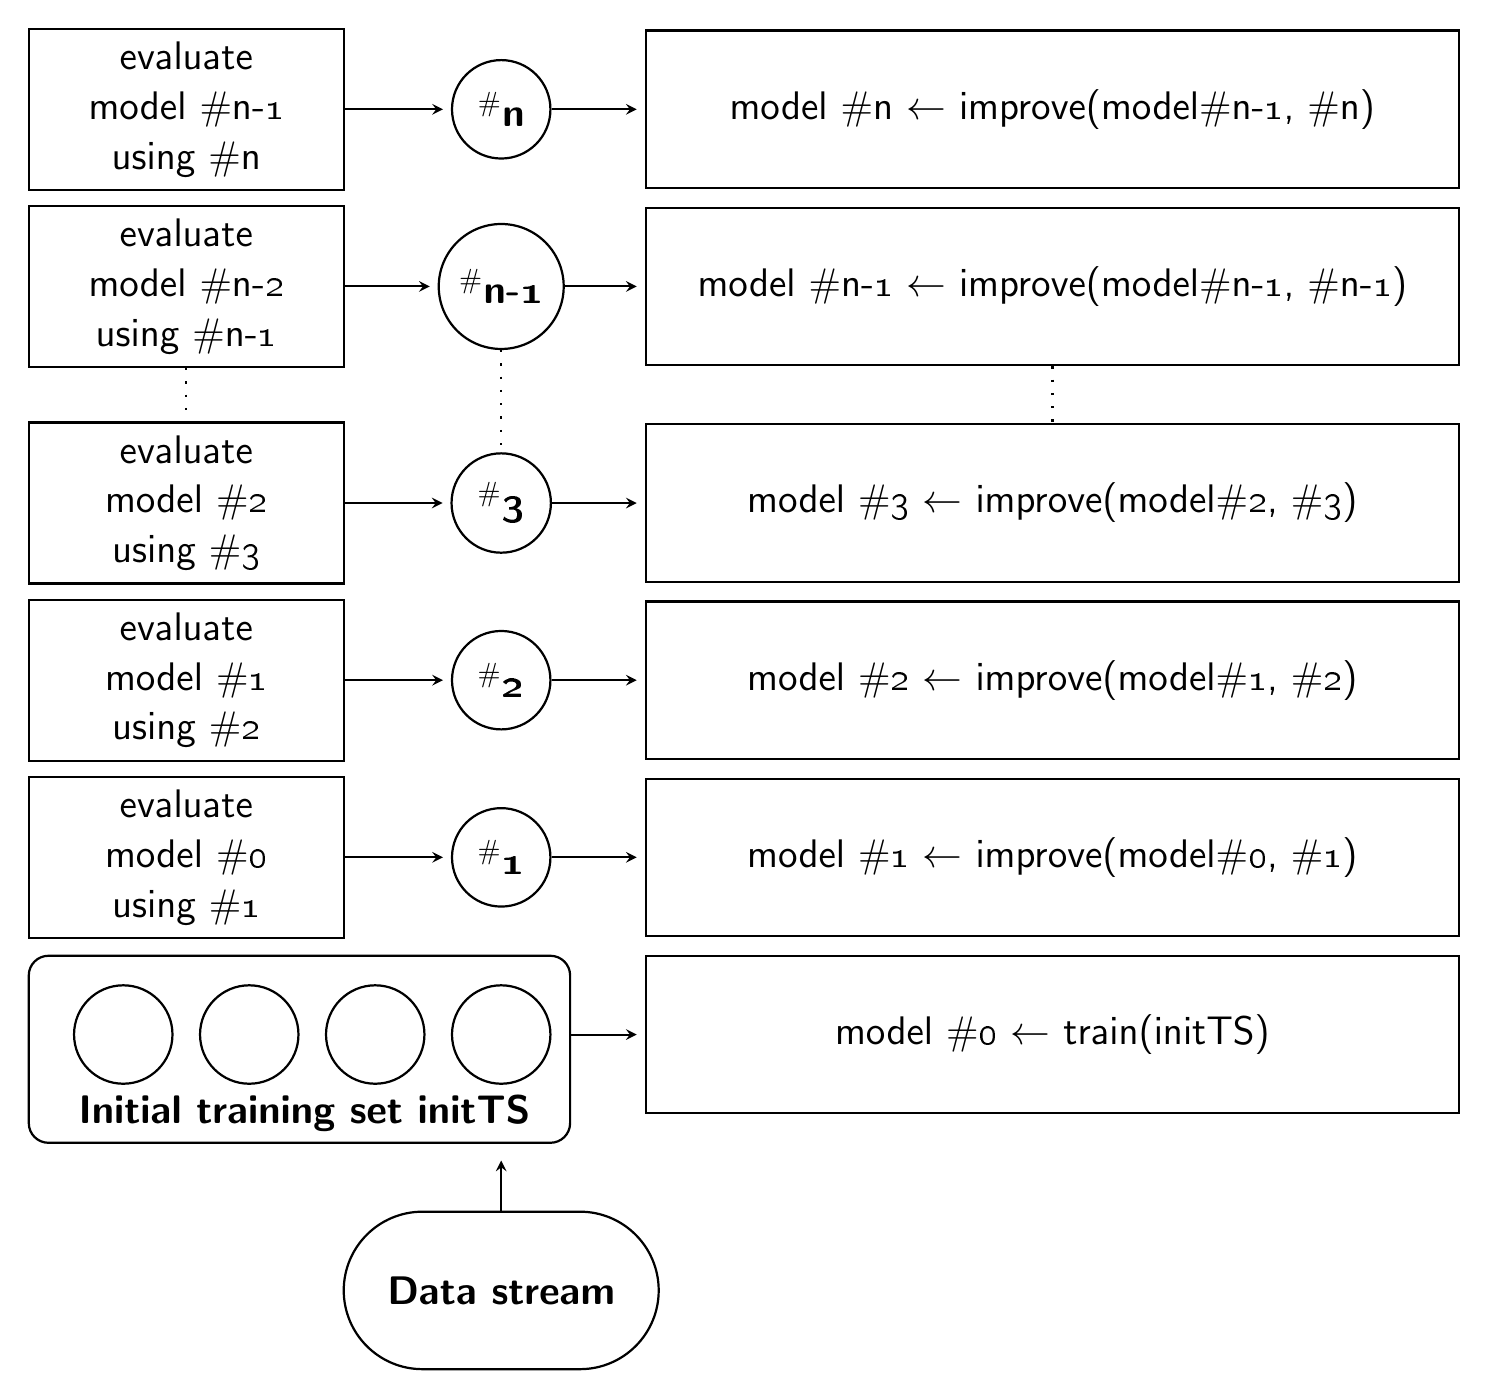
\begin{tikzpicture}[auto, thick, node distance=2cm, font=\sffamily]
\Large
\tikzset{%
	contra/.style = {black, fill = white, text=black},
	ds/.style = {draw,rectangle, minimum height = 2cm, minimum width = 4cm, rounded corners = 1cm, contra},
	chunk/.style = {draw,circle, minimum height = 1.25cm, minimum width = 1.25cm, contra},
	eval/.style = {draw,rectangle, minimum height = 2cm, minimum width = 4cm, text width=2.5cm, align = center},
	model/.style = {draw,rectangle, minimum height = 2cm, minimum width = 10cm, text width=10cm, align = center},
	con/.style = {->,shorten >=1mm,line width=.25mm,>=stealth}
}

% Data stream

\draw node at (0,-3) [chunk] (c1) {\bfseries $^\#$n}; 
\draw node at (0,-5.25) [chunk] (c2) {\bfseries $^\#$n-\oldstylenums1}; 
\draw node at (0,-8) [chunk] (c3) {\bfseries $^\#$\oldstylenums3}; 
\draw node at (0,-10.25) [chunk] (c4) {\bfseries $^\#$\oldstylenums2}; 
\draw node at (0,-12.5) [chunk] (c5) {\bfseries $^\#$\oldstylenums1};

\draw node at (-4,-3) [eval] (e1)
{evaluate model \#n-\oldstylenums1 \hspace{2em}using \#n}; 
\draw node at (-4,-5.25) [eval] (e2)
{evaluate model \#n-\oldstylenums2 \hspace{2em}using \#n-\oldstylenums1}; 
\draw node at (-4,-8) [eval] (e3)
{evaluate model \#\oldstylenums2 \hspace{2em}using \#\oldstylenums3}; 
\draw node at (-4,-10.25) [eval] (e4)
{evaluate model \#\oldstylenums1 \hspace{2em}using \#\oldstylenums2}; 
\draw node at (-4,-12.5) [eval] (e5)
{evaluate model \#\oldstylenums0 \hspace{2em}using \#\oldstylenums1}; 

\draw node at (7,-3) [model] (m1)
{model \#n $\leftarrow$ improve(model\#n-\oldstylenums1, \#n)};
\draw node at (7,-5.25) [model] (m2) 
{model \#n-\oldstylenums1 $\leftarrow$ improve(model\#n-\oldstylenums1, \#n-\oldstylenums1)};
\draw node at (7,-8) [model] (m3) 
{model \#\oldstylenums3 $\leftarrow$ improve(model\#\oldstylenums2, \#\oldstylenums3)};
\draw node at (7,-10.25) [model] (m4) 
{model \#\oldstylenums2 $\leftarrow$ improve(model\#\oldstylenums1, \#\oldstylenums2)};
\draw node at (7,-12.5) [model] (m5) 
{model \#\oldstylenums1 $\leftarrow$ improve(model\#\oldstylenums0, \#\oldstylenums1)};
\draw node at (7,-14.75) [model] (m6) 
{model \#\oldstylenums0 $\leftarrow$ train(initTS)};


\draw node at (-2.5,-15.75) {\bfseries Initial training set initTS};
\draw [rounded corners = .25cm] (-6,-13.75) rectangle (.875,-16.125);
\draw node at (-4.8,-14.75) [chunk] { };
\draw node at (-3.2,-14.75) [chunk] { }; 
\draw node at (-1.6,-14.75) [chunk] { }; 
\draw node at (0,-14.75) [chunk] { }; 

\draw node at (0,-18.0) [ds] (ds) {\bfseries Data stream};

\draw[con] (ds) -- (0,-16.25);
\draw[con] (e1) -- (c1);
\draw[con] (c1) -- (m1);
\draw[con] (e2) -- (c2);
\draw[con] (c2) -- (m2);
\draw[con] (e3) -- (c3);
\draw[con] (c3) -- (m3);
\draw[con] (e4) -- (c4);
\draw[con] (c4) -- (m4);
\draw[con] (e5) -- (c5);
\draw[con] (c5) -- (m5);
\draw[con] (.875,-14.75) -- (m6);

\draw[loosely dotted] (e2) -- (e3);
\draw[loosely dotted] (c2) -- (c3);
\draw[loosely dotted] (m2) -- (m3);

\end{tikzpicture}}
%		\vspace{1em}
%		\caption{Idea of \emph{Test and Train} evaluation.}	
%		\label{fig:testtrain}
%	\end{center}
%\end{figure}

\subsection{Results}
\label{subsec:exp:results}
\noindent Experiments were conducted with \oldstylenums{12} streams with three strategies:

\begin{itemize}
	\item Measuring accuracy of incrementally training a model with all samples available in data stream.
	\item Measuring accuracy of incrementally trained model with randomized chunk subset, according to a given budget with five values in range \oldstylenums{10}---\oldstylenums{90}\%.
	\item Measuring accuracy of incrementally trained model with active learning approach described in Section 2 with five values in range \oldstylenums{10}---\oldstylenums{90}\% for both given budget and threshold.
\end{itemize}

Because conducted experiments produced many learning curves, only the part of them is included in the paper, but the detailed experimental results may be found in the article repository\footnote{\url{https://github.com/w4k2/active_learning}}.

Figure \ref{fig:budget_learning_curve} shows, with a blue line, a learning curve for three different budget values (\oldstylenums{30}\%, \oldstylenums{50}\%, and \oldstylenums{70}\%), while the black line is a curve for the classifier trained on the basis of all labeled examples (budget = \oldstylenums{100}\%).

\begin{figure}[!ht]
	\begin{center}
		\resizebox {.32\columnwidth} {!} {\plotbudget{MLP100}{LED}{0.30}{0.30}{4cm}{1000}}		
		\resizebox {.32\columnwidth} {!} {\plotbudget{MLP100}{LED}{0.30}{0.50}{4cm}{1000}}		
		\resizebox {.32\columnwidth} {!} {\plotbudget{MLP100}{LED}{0.30}{0.70}{4cm}{1000}}
		\caption{Budget and learning curve}	
		\label{fig:budget_learning_curve}
	\end{center}
\end{figure}


Decreasing a given budget leads, similarly to increasing the chunk or reducing a structure, to reduce the dynamics of learning. Therefore, it can not be a sufficient practice to reduce the cost of labeling. To maintain the accuracy of learning on a smaller training set, it is necessary to select the appropriately reduced set of samples, which we try to achieve by the proposed active learning method.

For the same stream, Figure \ref{fig:treshold_learning_curve} shows, with a continuous red line, a learning curve for three different threshold values ($.1$, $.3$, and $.9$) with a fixed budget of \oldstylenums{70}\%. The black line is a curve for learning with all samples labeled, while the red dotted line is the percentage of samples used to train the model.

\begin{figure}[!ht]
	\begin{center}
		\resizebox {.32\columnwidth} {!} {\plotresult{MLP100}{LED}{0.10}{0.70}{4cm}{1000}}		
		\resizebox {.32\columnwidth} {!} {\plotresult{MLP100}{LED}{0.30}{0.70}{4cm}{1000}}		
		\resizebox {.32\columnwidth} {!} {\plotresult{MLP100}{LED}{0.90}{0.70}{4cm}{1000}}
		\caption{Treshold and learning curve}	
		\label{fig:treshold_learning_curve}
	\end{center}
\end{figure}


As we can see, too restrictive value of the threshold ($t = .1$) reduces the dynamics of the learning curve similarly to a low budget. The case of overly lax threshold ($t = .9$) allows to obtain the correct learning curve, but it does not reduce the samples necessary for the labeling, so it is no different from using only the budget parameter. However, proper calibration of the threshold ($t = .3$) allows to obtain the optimal learning curve, gradually reducing the need for sample labeling while obtaining knowledge by the classifier.

Figure \ref{fig:result_plots} shows the learning curves for selected, best parameters of a given budget and threshold for all tested data streams (continuous red lines). The black line is a curve for learning with all samples labeled. The red dotted line is the percentage of samples which were labeled during the model training.

\begin{figure}[!ht]
	\begin{center}
		\resizebox {.49\columnwidth} {!} {\plotresult{MLP100}{RBFGradualRecurring}{0.90}{0.90}{6cm}{1000}}
		\resizebox {.49\columnwidth} {!} {\plotresult{MLP100}{RBFNoDrift}{0.10}{0.90}{6cm}{1000}}
		\resizebox {.49\columnwidth} {!} {\plotresult{MLP100}{RBFBlips}{0.90}{0.90}{6cm}{1000}}
		\resizebox {.49\columnwidth} {!} {\plotresult{MLP100}{SEASuddenFaster}{0.30}{0.70}{6cm}{1000}}
		\resizebox {.49\columnwidth} {!} {\plotresult{MLP100}{SEASudden}{0.10}{0.30}{6cm}{1000}}
		\resizebox {.49\columnwidth} {!} {\plotresult{MLP100}{LEDNoDrift}{0.50}{0.90}{6cm}{1000}}
		\resizebox {.49\columnwidth} {!} {\plotresult{MLP100}{LED}{0.50}{0.90}{6cm}{1000}}
		\resizebox {.49\columnwidth} {!} {\plotresult{MLP100}{HyperplaneFaster}{0.50}{0.90}{6cm}{1000}}
		\resizebox {.49\columnwidth} {!} {\plotresult{MLP100}{HyperplaneSlow}{0.10}{0.70}{6cm}{1000}}
		\resizebox {.49\columnwidth} {!} {\plotresult{MLP100}{elecNormNew}{0.10}{0.90}{6cm}{448}}
		\resizebox {.49\columnwidth} {!} {\plotresult{MLP100}{covtypeNorm}{0.90}{0.90}{6cm}{5810}}
		\resizebox {.49\columnwidth} {!} {\plotresult{MLP100}{poker-lsn}{0.90}{0.10}{6cm}{8209}}
		\caption{Learning curves and label usages for selected, best parameters of a given budget and threshold for all tested data streams}	
		\label{fig:result_plots}
	\end{center}
\end{figure}





Table \ref{tab:results} presents a summary of the results obtained for the best combinations. It contains, for each data set, selected parameters, average accuracy for the model learned on the full and reduced stream, the difference between the accuracies and the percentage use of the stream.

\begin{table}[!ht]
\centering
\footnotesize
	\caption{A summary of the results obtained for the best combinations}
	\label{tab:results}
	\begin{tabular}{@{}nrrrrrr@{}}
	  \toprule
	    \multicolumn{1}{@{}N}{Data stream} & 
	    \multicolumn{2}{N@{}}{} &
	    \multicolumn{2}{N@{}}{Accuracies}\\
	  \cmidrule(lr){4-5}
	    &
	    \multicolumn{1}{c}{\scriptsize $t$} & 
	    \multicolumn{1}{c}{\scriptsize $b$} & 
	    \multicolumn{1}{c}{\scriptsize full} & 
	    \multicolumn{1}{c}{\scriptsize active} & 
	    \multicolumn{1}{c}{\scriptsize difference} & 
	    \multicolumn{1}{c@{}}{\scriptsize usage} \\
	  \cmidrule(r){1-1}\cmidrule(lr){2-2}\cmidrule(lr){3-3}\cmidrule(lr){4-4}\cmidrule(lr){5-5}\cmidrule(lr){6-6} \cmidrule(l){7-7}
\emph{RBFGradualRecurring} & .9 & 9 & 0.677 & 0.653 & $-0.025$ & 88.8\%\\
\emph{RBFBlips} & .9 & 9 & 0.773 & 0.725 & $-0.048$ & 79.2\%\\
\emph{HyperplaneFaster} & .5 & 9 & 0.834 & 0.826 & $-0.008$ & 52.0\%\\
\emph{LEDNoDrift} & .5 & 9 & 0.491 & 0.477 & $-0.013$ & 42.8\%\\
\emph{HyperplaneSlow} & .1 & 7 & 0.837 & 0.868 & $0.030$ & 39.9\%\\
\emph{LED} & .5 & 9 & 0.490 & 0.482 & $-0.008$ & 39.5\%\\
\emph{SEASuddenFaster} & .3 & 7 & 0.833 & 0.828 & $-0.005$ & 39.2\%\\
\emph{RBFNoDrift} & .1 & 9 & 0.807 & 0.817 & $0.010$ & 34.5\%\\
\emph{covtypeNorm} & .9 & 9 & 0.734 & 0.719 & $-0.015$ & 29.2\%\\
\emph{SEASudden} & .1 & 3 & 0.829 & 0.842 & $0.013$ & 22.4\%\\
\emph{poker-lsn} & .9 & 1 & 0.563 & 0.558 & $-0.005$ & 10.3\%\\
\emph{elecNormNew} & .1 & 9 & 0.623 & 0.577 & $-0.046$ & 2.3\%\\
	  \bottomrule
	\end{tabular}
\end{table}


\subsection{Analysis of the results}
\label{subsec:exp:analysis}

\noindent Most of the observations discussed around the Figures \ref{fig:budget_learning_curve} and \ref{fig:treshold_learning_curve} are confirmed by curves available in the Figure \ref{fig:result_plots}. We need to reject the \emph{elecNormNew} dataset, where even training with the fully labeled dataset led to a model with results similar to a random classifier.
%PAWEŁ CZY POWYŻEJ CHODZIŁO CI O RANDOM CLASSIFIER -CZY O TAKI, KTÓRY JEST FULL SUPERVISED
%ODP. Chodziło mi właśnie o klasyfikator losowy, a więc random classifier.
It is worth mentioning that Zliobaite \cite{Zliobaite:2013} observes the problem of testing data stream classifiers on autocorrelated data and that getting high accuracy, especially on the \emph{elecNormNew} dataset does not necessarily mean that the adaptation mechanism work well. 

In every dataset, after this exclusion, a tendency to consequently reducing the chunk usage is observed. In the case streams with many concept drifts (\emph{RBFGradualRecurring} and \emph{RBFBlips}) the reduction of label use is relatively small, but it is caused by a slow accumulation of knowledge of the selected classifier, where \oldstylenums{100} neurons in the hidden layer were not sufficient to achieve the maximum accuracy of classification before the next drift. We may also observe the intensive growth of the label demand, when a concept drift appears.

For data streams generated by \emph{Streaming Ensemble Algorithm}, the reduction of the accuracy is not observed. In the case of two sets of data (\emph{SEASudden} and \emph{HyperplaneSlow}), the appropriate combination of a given budget and threshold allows not only to preserve the dynamics of learning, but also to accelerate it.

Even in the case of data streams where the selected neural network structure was insufficient to achieve full discriminative power before occurrence of the next drift, it was possible to reduce the number of samples necessary for labeling by \oldstylenums{10}--\oldstylenums{20}\%. In the case of the remaining sets, a reduction of \oldstylenums{50}--\oldstylenums{90}\% was achieved, without a negative impact on the average quality of the classification.

\subsection{Lessons learned}
Let us summarize the research findings and observations that could be drawn from the experimental analysis:
\begin{itemize}
	\item Active learning approach may lead to a solution where a trained model keeps the classification accuracy of full-stream learning, with a slight reduction of used labels.
	\item There is no rule of correct setting the parameters related to a given budget and threshold, so it should be calibrated for a particular task.
	\item Active learning approach is able to detect a concept drift and react on it without negative impact on classification accuracy.
	\item Chunk usage decreases slowly in time, according to stabilization of a model on current concept.
	\item Acquiring the necessary knowledge by a model reduces the need for new samples.
	%PAWEŁ WYJAŚNIJ PONIŻSZE POJĘCIE KNOWLEDGE SATURATION
	%ODP. Przez nasycenie wiedzą miałem na myśli stopień uzyskania maksymalnej mocy dyskryminacyjnej. 
    \item A \emph{knowledge saturation} (degree of obtaining the maximum discriminative power) of a model can be successfully measured by \textsc{rfsd}.
    %PAWEŁ PONIŻSZA UWAGA JEST DOŚĆ POKRĘTNA, ZASTANÓW SIĘ< CZY JEJ NIE USUNĄĆ
    %ODP. Z przykładu z rysunku 5 wynikało początkowo, że być może wypadałoby całkowicie zrezygnować z budżetu, bo to przez próg najłatwiej kalibruje się aktywny klasyfikator. W niektórych przypadkach (właśnie tych dwóch) jednak widać, że połączenie obu ograniczeń czasami pozwala na polepszenie krzywej uczenia. Ale usunę uwagę, bo faktycznie nie do końca potrafię to wyjaśnić. 
	%\item The budget parameter is not unnecessary when using the threshold, because it can be seen that in some cases (HyperplaneSlow, SEASudden) and with a suitably matched threshold, it can even improve the learning curve in relation to the use of all patterns.
	\item Chunk reduction has a positive effect by increasing the learning frequency but extends the learning time itself.
    %PAWEŁ PONIŻSZE DWIE UWAGI PRZEISAŁEM - ZOBACZ, CZY WG CIEBIE JEST TERAZ OK, CZY COŚ  DODAĆ
    % ODP. Moim zdaniem jest teraz OK.
%	\item The greater the number of neurons, the higher accuracy decreases when the concept drifts.
%	\item Appropriate increase in the number of neurons allows the immunization of the model to accuracy decreases occurring at the incremental drift.
 \item The size of a neural network which is responsible for the concept memorization should be set carefully, for a given decision task, because on the one hand the smaller structure of the network the faster is its reaction to the concept drift, what is especially important in the case of sudden drift. Such fast model adaptation protect against the huge classification accuracy drop. On the other hand appropriate increasing of neural network size allows the immunization of the model to accuracy drop when the slow, incremental concept drift goes ahead. 
 	%PAWEŁ WYJAŚNIJ/ROZSZERZ PONIŻSZE.
 	%ODP. Chodzi mi właśnie o obserwację z rys 5, gdzie zmiejszenie przez budżet -- losowy podzbiór, spłaszcza krzywą uczenia. 
	\item Limitation of training set by just a given budget with random subset of samples causes a proportional reduction in the learning dynamics.
\end{itemize}

\label{subsec:exp:ll}